\chapter{Latex-Beispiele}
\label{chap:Beispiele}

\section{Bild}
\label{sec:Bild}
An dieser Stelle wird ein Beispiel zur Einbindung eines Bildes in Latex gegeben. 
\begin{figure}[htbp] %von Latex voreigestellt ist die Reihenfolge: tbp= top,bottom, page
\begin{center}
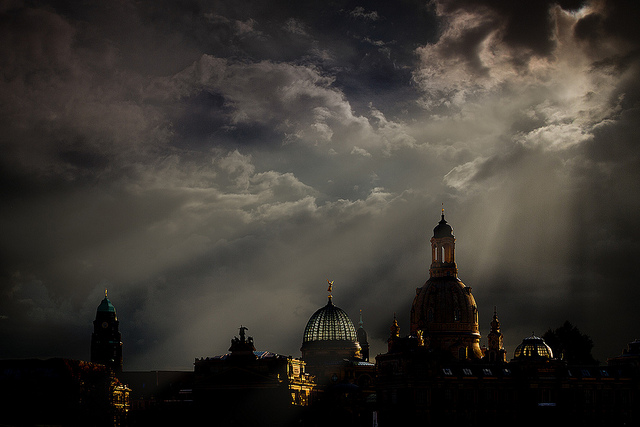
\includegraphics[width=0.5\textwidth]{img/Bild} % Bild im Ordner "img" (bei .jpg, .png, .pdf ist keine Dateiendung erforderlich)
\end{center}
\caption[Beispielbild]{Beispielbild [copyright flickr-user *Light Painting*] }
\label{fig:multpraef}
\end{figure}


\section{Tabelle}
\label{sec:Tabelle}

Dies ist eine sehr einfache Beispieltabelle ohne Gleitumgebung und dadurch ohne die Möglichkeit einer Tabellenunterschrift:
\begin{center}
	\begin{tabular}{lcr}
	\toprule
	Messung $n$ & Wert $a_1$ & Wert $a_2$\\
	\midrule
	1 & 6 & 5\\
	\midrule
	2 & 8 & 2\\
	\midrule
	3 & NaN & 1\\
	\midrule
	4 & 0 & ungültig \\
	\bottomrule
	\end{tabular}
\end{center}
\clearpage %Erzeugt neue Seite und gibt vorher alle Gleitobjekte aus.

%\noindent verhindert die Einrückung
\noindent Die empfohlene und in der Praxis gebräuchlichste Einbindung einer Tabelle: 
\begin{table}[htbp]
	\centering
	\begin{tabular}{lcr}
		\toprule
		Messung $n$ & Wert $a_1$ & Wert $a_2$\\
		\midrule
		1 & 6 & 5\\
		\midrule
		2 & 8 & 2\\
		\midrule
		3 & NaN & 1\\
		\midrule
		4 & 0 & ungültig \\
		\bottomrule
	\end{tabular}
	\caption{Eine Tabelle.} \label{tab:EineTabelle}
\end{table}
\medskip %vertikaler zusätzlicher Abstand, auch möglich: \smallskip \bigskip

\noindent Die folgende Tabelle ist in eine Gleitumgebung eingebunden, mit einer Tabellenüberschrift sowie einem komplexeren Design ausgestattet:
\begin{center}
{\footnotesize %Alt1
	\begin{longtable}{lrrr}
	\caption[Beispieltabelle]{Beispieltabelle}\\
	\toprule
	 & \multicolumn{3}{c}{\textbf{Text}}\\ 
	\cmidrule(r){2-4}
	\textbf{Wort} & 1 & 2 & 3 \\ 
	\midrule
	\endhead
	Wort & 1 & 2 & 3\\ 
	Wort & 4 & 5 & 6 \\ 
	Wort& 7 & 8 & 9 \\ 
	\bottomrule
	\endlastfoot
	\end{longtable} \label{tab:BeispTab}
}
\end{center}


\section{Verweis}
\label{sec:Verweis}
Hier ist ein Beispiel für das Verweisen auf Schriftstücke:
Siehe \cite{einbuch}, S. 84--89.

Der Verweis auf eine Tabelle, ein Bild oder anderes Kapitel wird dagegen wie folgt eingebunden: z.\,B. Tabelle~\ref{tab:BeispTab}, Bild~\ref{fig:multpraef} oder Abschnitt~\ref{sec:Bild}
% \,=ein vor Trennung geschützter geringerer Anstand ~=ein vor Trennung geschützter normaler Abstand

\section{Formeln}
\label{sec:Formeln}
Hier wird ein Beispiel zur Erstellung von Formeln gegeben.\footnote{So setzt man Fußnoten}

\begin{equation} U[X_{i},S_{n}] \geq U[X_{j},S_{n}] \ \ \forall j \qquad i > j \ \ \forall j \in \mathbf{C}
\end{equation}
wobei \\ 
\begin{tabular}{ll}
$U $ & Nutzen einer Alternative,\\
$X_{i}$ und $X_{j} $ & Attribut-Vektoren, die die Alternativen $i$ und $j$ beschreiben,\\
$S_{n} $ & Vektor, der die die Entscheidung beeinflussenden Eigenschaften des \\
& Entscheidungsträgers t beschreibt und\\
$\mathbf{C} $ & Alternativenmenge.
\end{tabular}
